%package list
\documentclass{article}
\usepackage[top=3cm, bottom=3cm, outer=3cm, inner=3cm]{geometry}
\usepackage{multicol}
\usepackage{graphicx}
\usepackage{url}
%\usepackage{cite}
\usepackage{hyperref}
\usepackage{array}
%\usepackage{multicol}
\newcolumntype{x}[1]{>{\centering\arraybackslash\hspace{0pt}}p{#1}}
\usepackage{natbib}
\usepackage{pdfpages}
\usepackage{multirow}
\usepackage[normalem]{ulem}
\useunder{\uline}{\ul}{}
\usepackage{svg}
\usepackage{xcolor}
\usepackage{listings}
\lstdefinestyle{ascii-tree}{
    literate={├}{|}1 {─}{--}1 {└}{+}1 
  }
\lstset{basicstyle=\ttfamily,
  showstringspaces=false,
  commentstyle=\color{red},
  keywordstyle=\color{blue}
}
%\usepackage{booktabs}
\usepackage{caption}
\usepackage{subcaption}
\usepackage{float}
\usepackage{array}

\newcolumntype{M}[1]{>{\centering\arraybackslash}m{#1}}
\newcolumntype{N}{@{}m{0pt}@{}}


%%%%%%%%%%%%%%%%%%%%%%%%%%%%%%%%%%%%%%%%%%%%%%%%%%%%%%%%%%%%%%%%%%%%%%%%%%%%
%%%%%%%%%%%%%%%%%%%%%%%%%%%%%%%%%%%%%%%%%%%%%%%%%%%%%%%%%%%%%%%%%%%%%%%%%%%%
\newcommand{\itemEmail}{rcompanocca@unsa.edu.pe}
\newcommand{\itemStudent}{Roni Companocca Checco}
\newcommand{\itemCourse}{Programación}
\newcommand{\itemCourseCode}{20210558}
\newcommand{\itemSemester}{II}
\newcommand{\itemUniversity}{Universidad Nacional de San Agustín de Arequipa}
\newcommand{\itemFaculty}{Facultad de Ingeniería de Producción y Servicios}
\newcommand{\itemDepartment}{Departamento Académico de Ingeniería de Sistemas e Informática}
\newcommand{\itemSchool}{Escuela Profesional de Ingeniería de Sistemas}
\newcommand{\itemAcademic}{2023 - B}
\newcommand{\itemInput}{Del 22 Diciembre 2023}
\newcommand{\itemOutput}{Al 23 Diciembre 2023}
\newcommand{\itemPracticeNumber}{03}
\newcommand{\itemTheme}{Herencia - Ejercicio 02}
%%%%%%%%%%%%%%%%%%%%%%%%%%%%%%%%%%%%%%%%%%%%%%%%%%%%%%%%%%%%%%%%%%%%%%%%%%%%
%%%%%%%%%%%%%%%%%%%%%%%%%%%%%%%%%%%%%%%%%%%%%%%%%%%%%%%%%%%%%%%%%%%%%%%%%%%%

\usepackage[english,spanish]{babel}
\usepackage[utf8]{inputenc}
\AtBeginDocument{\selectlanguage{spanish}}
\renewcommand{\figurename}{Figura}
\renewcommand{\refname}{Referencias}
\renewcommand{\tablename}{Tabla} %esto no funciona cuando se usa babel
\AtBeginDocument{%
	\renewcommand\tablename{Tabla}
}

\usepackage{fancyhdr}
\pagestyle{fancy}
\fancyhf{}
\setlength{\headheight}{30pt}
\renewcommand{\headrulewidth}{1pt}
\renewcommand{\footrulewidth}{1pt}
\fancyhead[L]{\raisebox{-0.2\height}{
\includegraphics[width=3cm]{logo_episunsa.png}}}
\fancyhead[C]{\fontsize{7}{7}\selectfont	\itemUniversity \\ \itemFaculty \\ \itemDepartment \\ \itemSchool \\ \textbf{\itemCourse}}
\fancyhead[R]{\raisebox{-0.2\height}{
\includegraphics[width=1.2cm]{abet.png}}}
\fancyfoot[L]{Estudiante Roni Companocca Checco}
\fancyfoot[C]{\itemCourse}
\fancyfoot[R]{Página \thepage}

% para el codigo fuente
\usepackage{listings}
\usepackage{color, colortbl}
\definecolor{dkgreen}{rgb}{0,0.6,0}
\definecolor{gray}{rgb}{0.5,0.5,0.5}
\definecolor{mauve}{rgb}{0.58,0,0.82}
\definecolor{codebackground}{rgb}{0.95, 0.95, 0.92}
\definecolor{tablebackground}{rgb}{0.8, 0, 0}

\lstset{frame=tb,
	language=bash,
	aboveskip=3mm,
	belowskip=3mm,
	showstringspaces=false,
	columns=flexible,
	basicstyle={\small\ttfamily},
	numbers=none,
	numberstyle=\tiny\color{gray},
	keywordstyle=\color{blue},
	commentstyle=\color{dkgreen},
	stringstyle=\color{mauve},
	breaklines=true,
	breakatwhitespace=true,
	tabsize=3,
	backgroundcolor= \color{codebackground},
}

\begin{document}
	
	\vspace*{10px}
	
	\begin{center}	
		\fontsize{17}{17} \textbf{ Informe de Teoria \itemPracticeNumber}
	\end{center}
	\centerline{\textbf{\Large Tema: \itemTheme}}
	%\vspace*{0.5cm}	

	\begin{flushright}
		\begin{tabular}{|M{2.5cm}|N|}
			\hline 
			\rowcolor{tablebackground}
			\color{white} \textbf{Nota}  \\
			\hline 
			     \\[30pt]
			\hline 			
		\end{tabular}
	\end{flushright}	

	\begin{table}[H]
		\begin{tabular}{|x{4.7cm}|x{4.8cm}|x{4.8cm}|}
			\hline 
			\rowcolor{tablebackground}
			\color{white} \textbf{Estudiante} & \color{white}\textbf{Escuela}  & \color{white}\textbf{Asignatura}   \\
			\hline 
			{\itemStudent \par \itemEmail} & \itemSchool & {\itemCourse \par Semestre: \itemSemester \par Código: \itemCourseCode}     \\
			\hline 			
		\end{tabular}
	\end{table}		
	
	\begin{table}[H]
		\begin{tabular}{|x{4.7cm}|x{4.8cm}|x{4.8cm}|}
			\hline 
			\rowcolor{tablebackground}
			\color{white}\textbf{Teoria} & \color{white}\textbf{Tema}  & \color{white}\textbf{Duración}   \\
			\hline 
			\itemPracticeNumber & \itemTheme & 04 horas   \\
			\hline 
		\end{tabular}
	\end{table}
	
	\begin{table}[H]
		\begin{tabular}{|x{4.7cm}|x{4.8cm}|x{4.8cm}|}
			\hline 
			\rowcolor{tablebackground}
			\color{white}\textbf{Semestre académico} & \color{white}\textbf{Fecha de inicio}  & \color{white}\textbf{Fecha de entrega}   \\
			\hline 
			\itemAcademic & \itemInput &  \itemOutput  \\
			\hline 
		\end{tabular}
	\end{table}

    \section{EQUIPOS, MATERIALES Y TEMAS UTILIZADOS}
	\begin{itemize}
		\item Sistema Operativo Windows
		\item OpenJDK 64-Bits 17.0.7.
		\item Git 2.39.2.	
  	\item Cuenta en GitHub con el correo institucional.
	\end{itemize}

    \section{URL DE REPOSITORIO GITHUB}
	\begin{itemize}
		\item URL para el Repositorio GitHub.
		\item \url{https://github.com/RONI-COMPANOCCA-CHECCO}
		\item URL para el laboratorio 22 en el Repositorio GitHub.	
        \item \url{https://github.com/RONI-COMPANOCCA-CHECCO/FP2-TRABAJO03/tree/master/trabajo03/Ejercicio2.java}
	\end{itemize}
    
    \section{Ejercicio 02:}
	\begin{itemize}
        \item Utilizando la clase construida en el ejercicio 01, obtener una clase derivada Cilindro derivada de Circulo. La clase Cilindro deberá tener una función miembro que calcule la superficie de dicho cilindro. La fórmula que calcula la superficie del cilindro es S = 2r(l + r) donde r es el radio del cilindro y l es la longitud.
        \item Codigo
        \item clase Cilindro.java
        \begin{lstlisting}[language=java]
// RONI COMPANOCCA CHECCO
// FP2 - TRABAJO 03
// CUI 20210558
class Cilindro extends Circulo {
    double longitud;
    // REALIZAMOS EL SIGUIENTE CONSTRUCTOR
    public Cilindro(double centroX, double centroY, double radio, double longitud) {
        super(centroX, centroY, radio);
        this.longitud = longitud;
    }
    // Este método calcularSuperficie() en la clase Cilindro sirve para calcular la superficie de un cilindro.
    public double calcularSuperficie() {
        return 2 * Math.PI * this.radio * (this.longitud + this.radio);
    }
}
        \end{lstlisting}

        \item clase Main.java
        \begin{lstlisting}[language=java]
// RONI COMPANOCCA CHECCO
// FP2 - TRABAJO 03
// CUI 20210558
public class Main {
    public static void main(String[] args) {
        // Este código se utiliza para crear dos instancias
        Punto punto1 = new Punto(1, 2);
        Punto punto2 = new Punto(4, 6);
        // esta linea invoca un método llamado distancia en el objeto punto1 de la clase Punto. 
        double distanciaEntrePuntos = punto1.distancia(punto2);
        System.out.println("Distancia entre los puntos: " + distanciaEntrePuntos);
        // Esta línea de código crea una nueva instancia de la clase Circulo 
        Circulo circulo = new Circulo(0, 0, 5);
        System.out.println("Área del círculo: " + circulo.obtenerArea());
        // agregamos esta nueva linea de codigo para invocar la clase cilindro
        Cilindro cilindro = new Cilindro(0, 0, 5, 10);
        System.out.println("Superficie del cilindro: " + cilindro.calcularSuperficie());
    }
}
        \end{lstlisting}

        \item Cuando ejecutamos los codigos lo que nos sale como respuesta es la siguiente, calculamos la distacia de dos puntos, el area del circulo y tambien nos calcula la suerficie del cilindro.
        \centering
        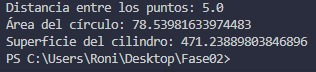
\includegraphics[height=3.5cm]{ima1.jpeg}
        \item si lo resolvemos matematicamente la superficie del cilindro con la formula que nos dieron pues tambien sale el mismo resultado, por lo cual llegamos a la conclusion de que nuestro codigo esta funcionando correctamente.
        \item .
        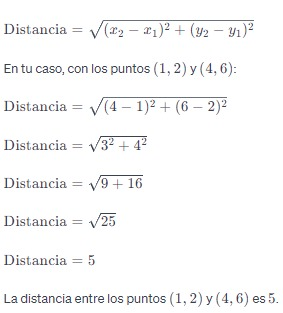
\includegraphics[height=8cm]{ima2.jpeg}
        
	\end{itemize}

	\section{REFERENCIAS}
	\begin{itemize}
		\item M. Aedo, “Fundamentos de Programación 2 - Tópicos de Programación Orientada a Objetos”, Primera Edición, 2021, Editorial UNSA.
		\item \url{https://github.com/rescobedoq/programacion.git}
		\item J. Dean, "Introduction to programming with Java: A Problem Solving Approach”, Third Edition, 2021, McGraw-Hill.
        \item C. T. Wu, "An Introduction to Object-Oriented Programming with Java", Fifth Edition, 2010, McGraw-Hill.
        \item P. Deitel, "Java How to Program", Eleventh Edition, 2017, Prentice Hall.
	\end{itemize}
	
%\clearpage
%\bibliographystyle{apalike}
%\bibliographystyle{IEEEtranN}
%\bibliography{bibliography}
			
\end{document}